\chapter{FDI}
\label{chap:FDI}


\section{The literature on Japanese MNCs investment}

Make a graph about the size of Japanese FDI relative to Asia FDI here

Calculate the size of Japanese FDI into several countries (nominator from JETRO,
denominator from IMF)

Relative exchange rate (Takagi2011). Assume that the capital market is
imperfect, that external borrowers face a premium. So if a host country currency
depreciates, inflow FDI will increase because the same amount of source currency
can buy more input in the host country. The relationship is especially strong
between exchange rate and inflow of FDI into industries with a lot of
firm-specific assets. (e.g. Japanese firms buy a US firm with innovation for
cheap, then use that innovation to improve its production back home in yen)

(Originally people don't think exchange rate matter because if you can buy an
asset for cheap in the host country, when you repatriate the profit back to the
home country it's a wash)

FDI is all about the relative factors (because a firm thinks about a country in
terms of how that country is relative to its host). So the two sided matching
framework makes sense

General FDI: Why don't firms export or license, but open their own plant
overseas? Argument is that they have firm-specific asset that cannot be fully
exploited otherwise. A licensee won't be able to exploit the entire asset, both
sides can't agree on a price beforehand (This is the OLI framework,
ownership-location-internalization, also the internationalization hypothesis).
Empirically, firm specific asset is unobservable, so people use R\&D intensity
and advertising intensity instead. R\&D does correlate strongly with
multinationality.


\section{Applying the Two-Sided Matching Model to Japanese MNCs}
\label{sec:application}

In this section, I apply the two-sided matching model to study the investment
location of Japanese firms overseas. The data comes from a dataset compiled by
Andrew Delios from \textit{Kaigai Shinshutsu Kigyou Souran} (Japanese Overseas
Investments-by Country), between 1986-1999 editions, a publication that contains
information about the foreign affiliates of listed Japanese firms.\footnote{I
thank Professor Andrew Delios for generously sharing the data.} Tokyo Keizai,
Inc. collect these data via annual surveys of the overseas operations of both
listed and non-listed firms. This database is reputed to include all Japanese
firms overseas \citep{Yamawaki1991}. \citep{Delios2001} compares the coverage of
the Japanese Overseas Investment with other sources of publicly listed firms and
found that 98.5\% of public firms are included, which has 99.5\% of the foreign
subsidiaries. Since there is no public information on non-public firms, they
cannot check the coverage of the Japanese Overseas Investment for these firms.
However, the result for the public firms makes us confident that our data is
close to the population of Japanese FDI overseas. This dataset has been used to
study X, Y, and Z \citep{Delios2000}. \footnote{There are similar datasets if
scholars want to replicate this study in other context. On a global scale, the
ORBIS dataset claims to have data of FDI firms across countries. (cite the paper
that I reviewed). However, there are concerns about its data quality, given that
the data is collected via public governmental or municipal sources. Due to the
differences of reporting across jurisdiction, the data quality is much less
consistent than the Japanese Overseas Survey. For the US, there is a census of
US firms overseas, which should be similarly high quality. However, this dataset
requires citizenship. Tokyo Keizai, Inc. also continue to publish this data
series. However, the cost is prohibitive and require understanding Japanese to
work with.}


(I use manufacturing FDI, so most capital in manufacturing is fixed) (because of
the the ``obsolescing bargaining'' argument. )



Sample choices:

- I only use the data of subsidiaries that are founded in year 1996 (which is
different from the list of companies who are in existence in year 1996).
Reasons: + the utility function is only modeled as a linear combinations of the
country / firms covariates. It does not take into account the cost of uprooting
a firm to move to another country once they are already there. This is important
for FDI because, unlike equity investor, FDI are less foot-loose. Indeed, the
fact that it is not footloose is an important quality of FDI that's appealing to
countries (cite). The political economy literature on FDI has also derived its
insights largely from this ``obsolescing bargain'' problem, so it's important
that our model takes this into account. In past applications of the two sided
matching approach, researchers use a random sample in time (i.e. a sample of all
couples who's married in a certain year), which is fine, because the cost of
leaving a job or leaving a partner may not be too onerous. However, for FDI,
this fixed cost is more central. By limiting the sample to the firms who are
founded in 1996, we examine their decisions as they are all looking for
potential locations.\footnote{Of course, a subsidiary's foundation year in 1996
does not preclude the decision process to happen outside of this year. However,
I consider this a reasonable approximation, given that many country
characteristics, especially the political and institutional ones, do not change
drastically within a window of several years.}

+ the data is largest for this year. (some summary statistics here). There may
be some concerns about this year being a special year, in the year leading up to
the 1997 Asian Financial Crisis. But 1) we're only looking at manufacturing
firms, not equity investors or land developers, 2) FDI during the crisis is
largely the same as before the crisis \citep{UNCTAD1998}. Indeed, this is
because FDI firms are largely looking at countries' fundamentals, such as labor
cost, market potential, and thus not affected by the fluctuations in the
financial markets. Essentially, the types of firms that invest before, during,
and after crisis are still the same types of firms.\footnote{One potential
concern is that our data does not capture the firms who thought about making an
investment but decided not to. This could be a problem if the MNCs in our
dataset is the most risk-seeking firms, then essentially we've only estimated
the preference of the very risk-seeking or the very risk-averse firms. AFC too
high short term interest, too high local currency that is fixed. However, the
exit rate of Japanese firms in Thailand, the epicenter of the financial crisis,
is the same, indicating that the types of firms who invest are not so affected
by the financial crisis. Looking at the exit is the reverse way of looking at
who would have invested but didn't. \citep{Delios2001}}

+ I only consider Japanese FDI into East Asian and Southeast Asian economies to
make sure that it's realistic to say that all these companies have the same
preference parameters. \citep{Pak2005} finds that Japanese FDI in the West seeks
to augment their global competitiveness, while Japanese FDI in the East focuses
on exploiting their core competencies. Japanese FDI in the West are ones with
oligopolistic power in their domestic market (so they are in a strong position
to compete) and require R\&D and marketing capabilities. They have different
level of equities. This suggests that the two types of firms are fundamentally
different.\footnote{Even though the difference in theory could be due to the
preference of the countries. However, it doesn't make sense why the level of
Japanese ownership is also different (because countries would not care about
this).}

The final sample includes 6474 Japanese foreign affiliates in 2003, spreading
across 37 countries, with China and the US leading as the two top destinations
for Japanese MNCs (Table \ref{tab:list_of_countries}).

For firms' characteristics that countries consider, I include:

\begin{itemize}
\item Capital size (in US\$): A main argument for the benefit of FDI is that it
brings capital to the country, improving labor productivity. MNCs' capital is
especially important for developing countries, which cannot muster much domestic
capital from their poor population. The capital size of a firm is included in
the Japanese Overseas Business dataset.

\item Labor size: Similarly, a reputed benefit of FDI is that it creates jobs,
generating not just economic growth but also increasing the government's
popularity among the populace. The total number of employees of a firm is
included in the Japanese Overseas Business dataset.

\item Technology intensity: I proxy for a firm's technology intensity by the
industry to which it belongs. \citet{OECD2009} categorizes ISIC industries into
four levels of technology intensity---low, medium low, medium high, and
high---according to the level of R\&D expenditure divided by sales. I convert
the industry classification of firms in my data from SIC 3 to ISIC and
categorize their technology intensity from 1 to 4, with 1 being low and 4 being
high. On several occasions, one industry in SIC 3 matches to multiple ISIC (rev
3) industries or none at all. In the former case, I take the average across
matched ISIC industries. In the latter case, the data is missing and later
removed from the analysis.\footnote{\cite{Bergstrand2007} discusses the
difference between R\&D intensity and advertising intensity, and find that R\&D
intensity is higher for manufacturing firms compared with consumer product
firms. Plus R\&D intensity is much more important for firms' performance than
advertising intensity.}\footnote{Definition of R\&D intensity: the amount spent
on R\&D as a percentage of sale}

\item Export intensity (ratio of export to sale):
\end{itemize}

Summary statistics table for these covariates.


For countries' characteristics that firms consider, I include:

\begin{itemize}
\item Market size: MNCs are expected to prefer countries with a large market
size, which present MNCs with many potential customers. Indeed, this has been
often cited as the allure of China to MNCs \citep{Luo2010}, as well as confirmed
in larger studies. This is also a major variable in the gravity model, which has
become a standard model for analyzing FDI flows. \citet{Bergstrand2007} provides
the theoretical framework for the use of gravity model. I follow the standards
in the literature and include log GDP (constant 2005 US\$), taken from the Penn
World Table.\footnote{An advantage of the Penn World Table is that it compiles
data for Taiwan, an important destination that the World Bank Development
Indicators does not include.}

\item Level of development: MNCs are expected to prefer countries with a high
level of development. A developed economy has consumers with high purchasing
power and better infrastructure. It can also measure capital abundance, in which
case a higher GDP per capita imply less flow because the simple model of FDI
frames FDI as the movement of capital from the capital rich countries to the
capital poor countries. To measure development, I use log GDP per capita
(constant 2005 US\$) from World Development Indicators.

\item GDP growth may be a proxy of potential returns,

\item Labor quality: As one primary factor of production, labor matters greatly
to firms' productivity and profit. To measure labor quality, I use the average
years of schooling of adult, taken from the UNDP's Human Development
Report.\footnote{Since Taiwan is not included in UNDP's and World Bank's data, I
collected its statistics from the Taiwanese Statistical Website.}

\item Democracy: Democracy has been a mainstay in the political science
literature on FDI. Scholars have argued that MNCs want to invest in democratic
regimes for various reasons, including stable policy, credible commitment, and
strong property rights \citep{Ahlquist2006, Li2003, Jensen2003}. On the other
hand, recent works have also argued that democratic regimes want FDI more than
autocratic regimes \citep{Pandya2016}. Thus, it is unclear whether the observed
high level of FDI in democracies is due to the push or the pull factors. By
controlling for countries' preference in the two-sided matching model, I can
better estimate the effect of democracies on firms' utility. I measure democracy
using the binary Demoracy \& Dictatorship, developed by \citet{Cheibub2009b}.
\end{itemize}

\section{Result}
\label{sec:result}

\begin{figure}[!ht] \centering
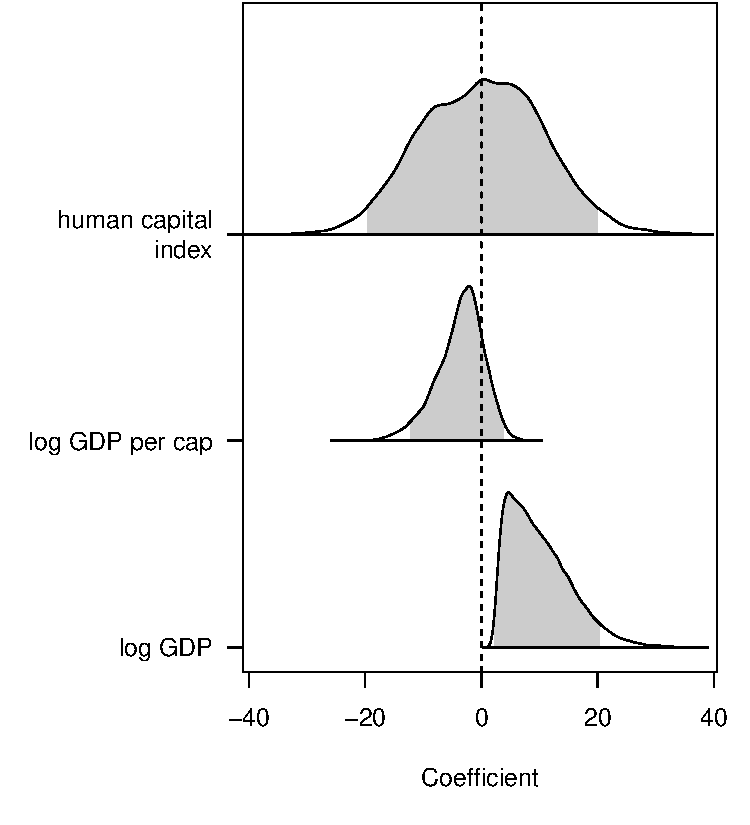
\includegraphics[width=0.75\textwidth,keepaspectratio]{japan96_alpha}
  \caption{Preference of MNCs for countries' characteristics. The density plot
and the shaded region show the posterior distribution and the 95\% credible
interval.}
  \label{fig:japan96_alpha}
\end{figure}

\begin{figure}[!ht] \centering
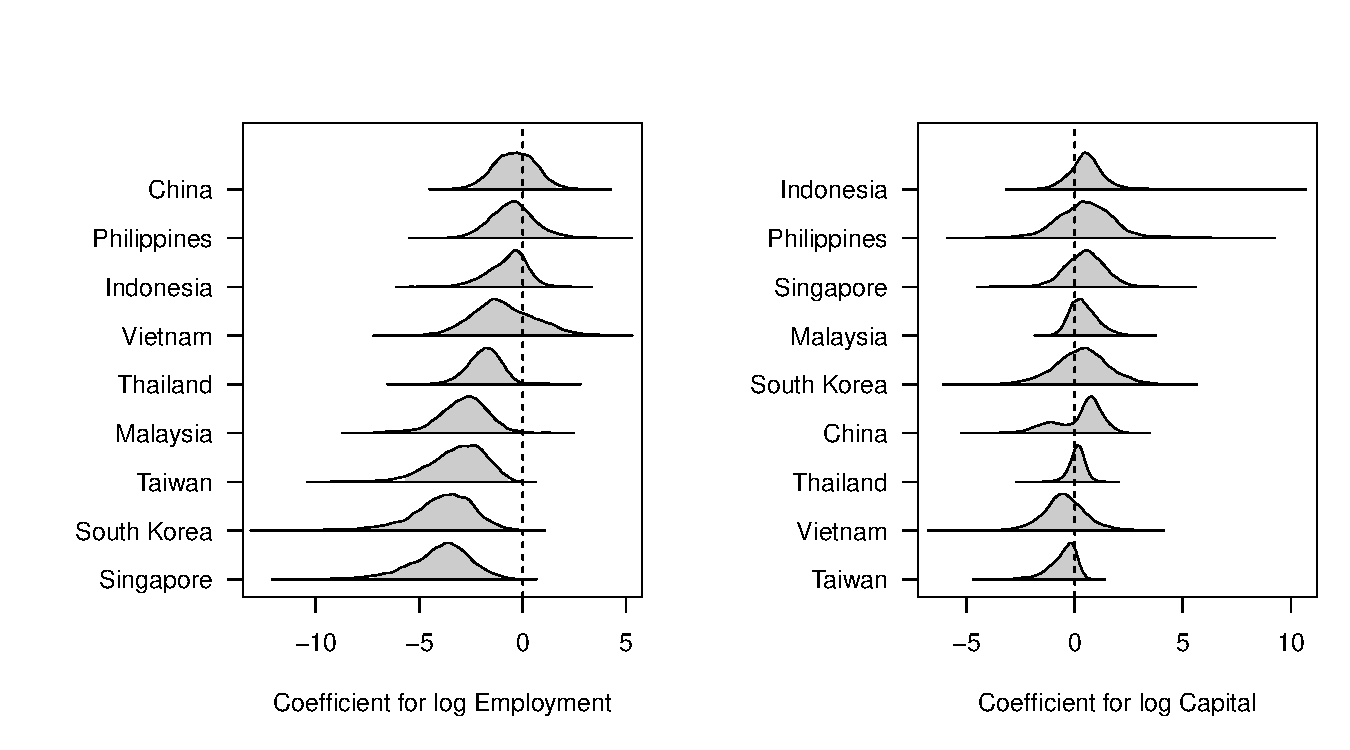
\includegraphics[width=\textwidth,keepaspectratio]{japan96_beta_ltemp_luscptl}
  \caption{Preference of countries for firms' size, measured by their labor
force (left) and capital (right). The density plot and the shaded region show
the posterior distribution and the 95\% credible interval.}
  \label{fig:japan96_beta_ltemp_luscptl}
\end{figure}

\begin{figure}[!ht] \centering
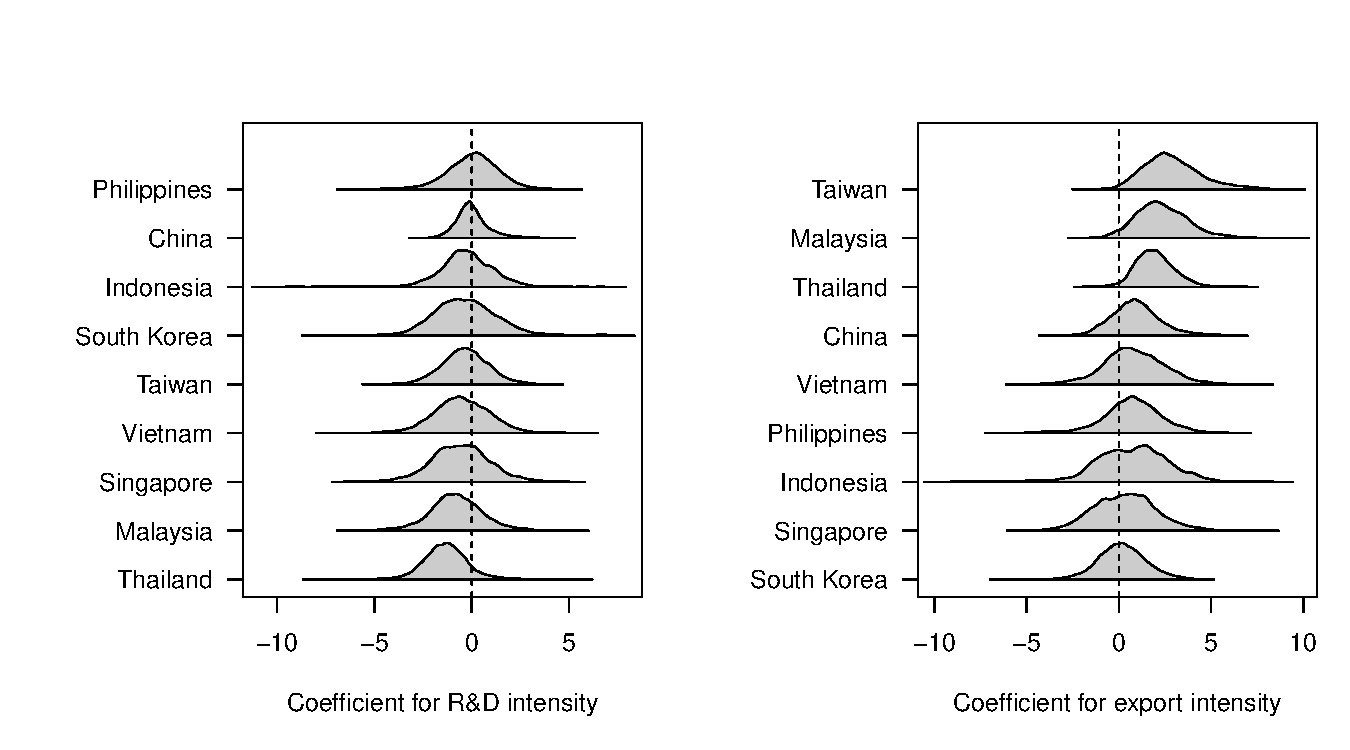
\includegraphics[width=\textwidth,keepaspectratio]{japan96_beta_intrd_intexp}
  \caption{Preference of countries for firms' intangible assets, i.e R\&D
intensity (left) and export intensity (right). The density plot and the shaded
region show the posterior distribution and the 95\% credible interval.}
  \label{fig:japan96_beta_intrd_intexp}
\end{figure}

\begin{figure}[!ht]
  \centering
  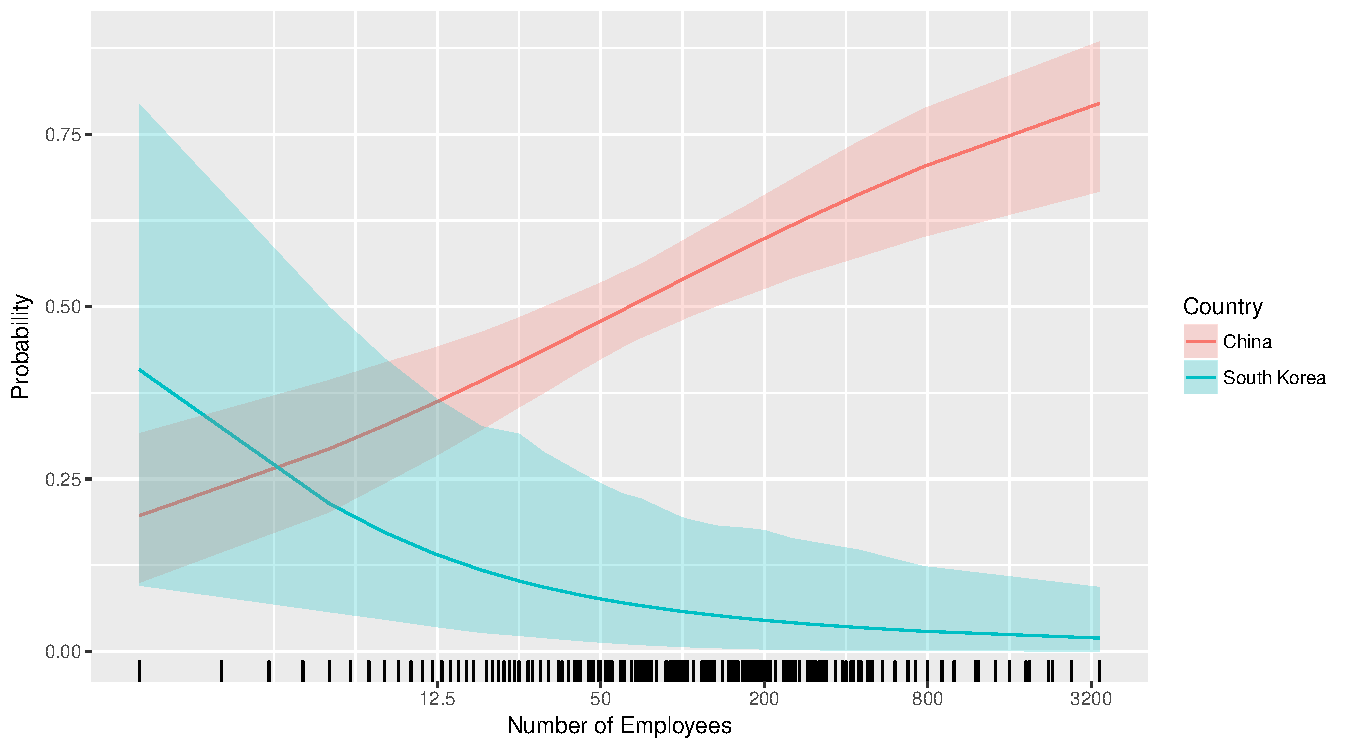
\includegraphics[width=\textwidth,keepaspectratio]{../figure/japan96_effect_of_temp}
  \caption{The effect of employee size on the probability to be offered by China
    and South Korea}
  \label{fig:japan96_effect_of_temp}
\end{figure}

\section{Model fit}
\label{sec:model_fit}

\begin{figure}[!ht] \centering
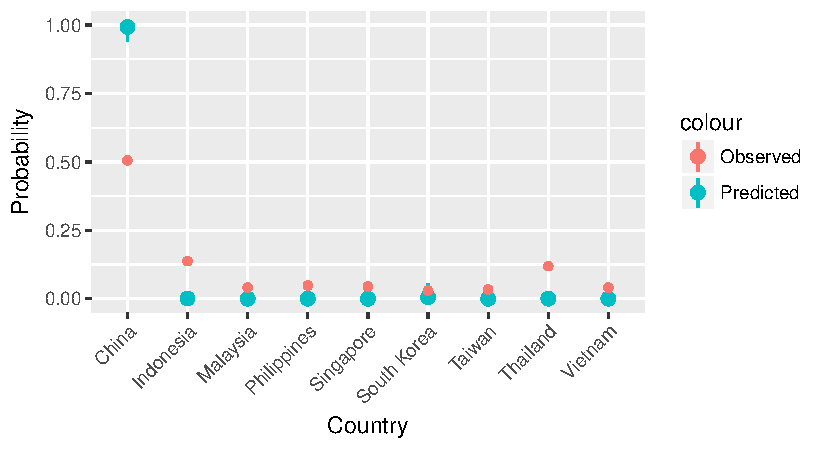
\includegraphics[width=\textwidth,keepaspectratio]{japan96_prob_being_chosen_by_MNC_one_sided}
  \caption{Predicted and observed probabilities that an MNC chooses to locate in
a country, unconditional on the preference of countries. The point and the error
bar show the posterior mean and the 95\% credible interval.}
  \label{fig:japan96_prob_being_chosen_by_MNC_one_sided}
\end{figure}


\begin{figure}[!ht] \centering
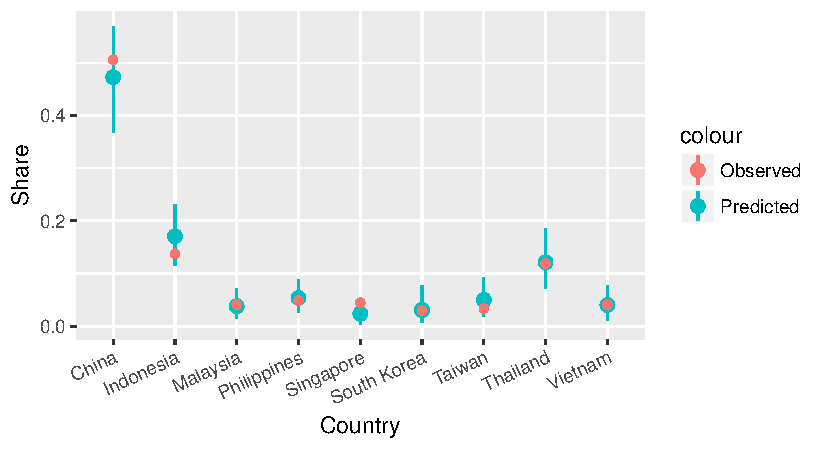
\includegraphics[width=\textwidth,keepaspectratio]{japan96_prob_being_chosen_by_MNC_two_sided}
  \caption{Predicted and observed probabilities that an MNC chooses to locate in
a country, conditional on the preference of countries. The point and the error
bar show the posterior mean and the 95\% credible interval.}
  \label{fig:japan96_prob_being_chosen_by_MNC_two_sided}
\end{figure}

Profiles of firms

\begin{figure}[!ht] \centering
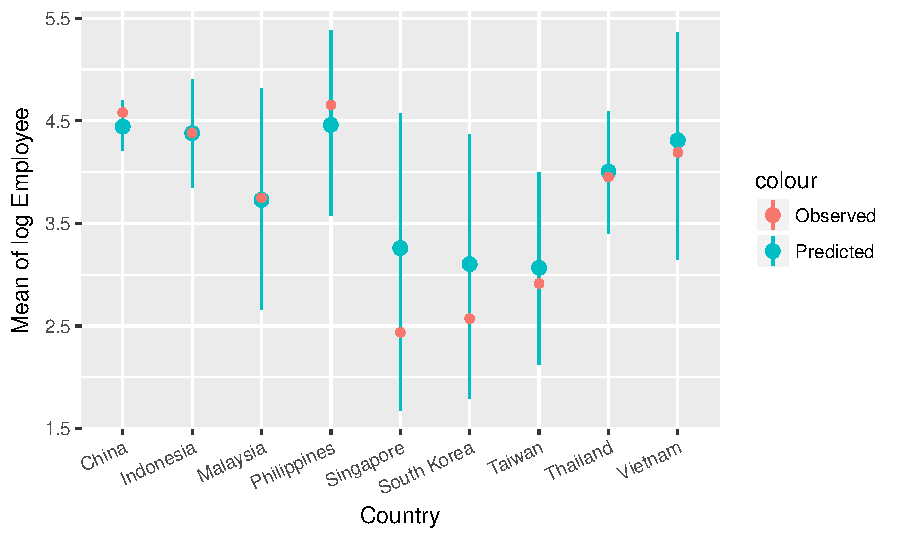
\includegraphics[width=\textwidth,keepaspectratio]{japan96_sim_mean_ltemp}
  \caption{Average of MNCs' labor size across countries. The point and the error
bar show the posterior mean and the 95\% credible interval.}
  \label{fig:japan96_sim_mean_ltemp}
\end{figure}

\begin{figure}[!ht] \centering
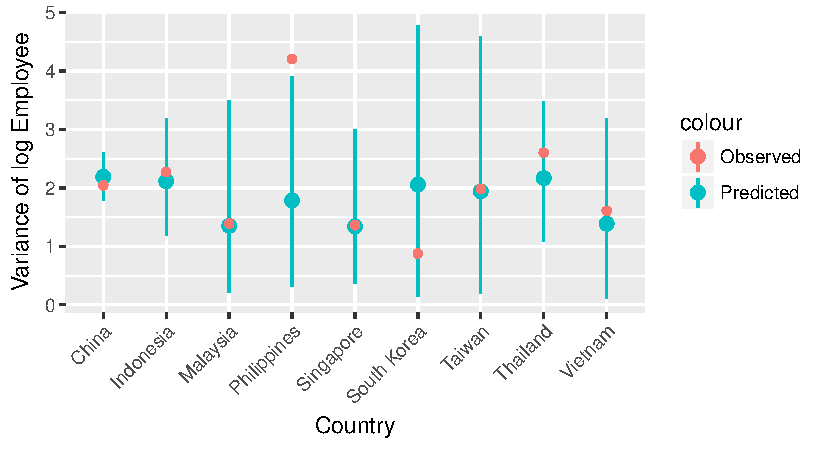
\includegraphics[width=\textwidth,keepaspectratio]{japan96_sim_var_ltemp}
  \caption{Variance of MNCs' labor size across countries. The point and the
error bar show the posterior mean and the 95\% credible interval.}
  \label{fig:japan96_sim_var_ltemp}
\end{figure}

\section{Political determinants of FDI}

\citep{Nunnenkamp2002} finds that for developing countries market based factors
are still the most important

\section{Conclusion}
\label{sec:conclusion}

In this paper, I propose the two-sided matching model to estimate firms' and
countries' preferences, solving three persistent issues in the literature of
FDI's political determinants. The results indicate that, for Japanese MNCs, only
a country's level of development matters and not its market size, labor quality,
or regime type. This finding suggests that we should take a closer look at the
relationship between democracies and MNCs. Since previous works in the
literature have not controlled for countries' preferences, they may have
mistaken democracies' love for FDI as FDI's fondness for democracies.

On the other hand, the model's estimation of countries' preference remains
lacking. Since each country has its own set of parameters, the parameter space
seems too large for the current implementation of the Metropolis-Hastings
algorithm to fully explore. Several solutions are possible. First, we can
collapse countries into categories of interest, e.g. regime types, (categorical)
time horizon length. Second, we can build a hierarchical model, modeling
countries' preferences as draws from a common distribution. Such model will
allow us to pool information across countries and reduce the parameter space.

%%% Local Variables:
%%% mode: latex
%%% TeX-master: "AnhLe_dissertation.tex"
%%% End: